\documentclass[12pt]{article}
\usepackage[utf8]{inputenc}
\usepackage[a4paper, margin=2cm]{geometry}
\usepackage[T1]{fontenc}
\usepackage{graphicx}
\usepackage{geometry}
\usepackage{amsmath}
\usepackage{amsfonts}
\usepackage{amssymb}
\usepackage{booktabs}
\usepackage{hyperref}
\usepackage{fancyhdr}
\usepackage{float}
\usepackage{ulem}
\usepackage{xeCJK}
\usepackage{listings}
\usepackage{xcolor}
\usepackage{indentfirst}
\setmainfont{Times New Roman}
\setCJKmonofont[BoldFont=SimHei, AutoFakeBold=true]{SimSun}
\lstset{
    basicstyle=\ttfamily\small,
    commentstyle=\color{gray},
    keywordstyle=\color{blue},
    stringstyle=\color{red},
    numberstyle=\tiny\color{gray},
    breaklines=true,
    captionpos=b,
    keepspaces=true,
    numbers=left,
    numbersep=5pt,
    showspaces=false,
    showstringspaces=false,
    showtabs=false,
    tabsize=2,
    frame=single,
    language=[x86masm]Assembler
}

\begin{document}
\thispagestyle{empty}

\begin{center}
    \vspace*{2cm}
    
    \Huge \textbf{2023-2024学年春季学期} \\
    \vspace{2cm}
    
    \Huge \textbf{《汇编语言程序设计》} \\
    \vspace{4cm}
    
    \large 评分：\underline{\hspace{4cm}} \\
    \vspace{6cm}
    
    \begin{tabular}{rl}
        \Large 学\hspace{2em}院： & \Large \underline{\makebox[12em][l]{\quad 计算机科学与工程学院}} \\
        \Large 专\hspace{2em}业： & \Large \underline{\makebox[12em][l]{\quad 计算机科学与技术}} \\
        \Large 班\hspace{2em}级： & \Large \underline{\makebox[12em][l]{\quad 计算机2204班}} \\
        \Large 姓\hspace{2em}名： & \Large \underline{\makebox[12em][l]{\quad 李俊洁}} \\
        \Large 学\hspace{2em}号： & \Large \underline{\makebox[12em][l]{\quad 20225443}} \\
        \Large 任课教师：         & \Large \underline{\makebox[12em][l]{\quad 刘思宇、柳秀梅}} \\
    \end{tabular}
    \vfill
\end{center}
\newpage

\section{实验目的}
实验的主要目的是加深对汇编语言程序设计的理解，通过具体的编程任务，掌握汇编语言的基本操作和技巧。
具体目标包括：
\begin{itemize}
    \item 理解和应用数据段的概念，学会如何在汇编语言中定义和操作数据。
    \item 学习使用循环和条件分支结构来处理数据，以实现复杂的逻辑判断和数据处理。
    \item 掌握如何通过汇编语言进行简单的数学计算，如求平均值，包括处理整数除法和相关的异常情况（如除零错误）。
    \item 熟悉如何通过DOS中断调用实现基本的输入输出操作，增强程序与用户的交互能力。
    \item 提高调试汇编语言程序的能力，通过实际的编程练习来解决问题并验证程序的正确性。
\end{itemize}

\section{实验要求}
本实验旨在通过编写和测试汇编程序来验证对汇编语言掌握的深度和准确性。实验的具体要求如下：
\begin{itemize}
    \item 编写汇编程序，该程序能够从预定义的内存区域读取字节数据，并根据这些数据计算出正数和负数的平均值。
    \item 在数据段中正确定义并初始化数据数组和其他必要的变量。数组的大小和元素值应该可以方便地修改以测试不同的数据集。
    \item 确保程序能够区分正数、负数和零，正确地计算出只包含正数或负数时的平均值，以及处理混合数据集。
    \item 程序需要能够处理可能的运行时错误，例如除零错误，并在这种情况下安全地终止或跳过错误处理。
    \item 在DOS环境下通过中断调用实现数据的输出，所有计算出的平均值都需要在屏幕上以适当的格式显示。
    \item 提交完整的源代码和详细的代码注释，解释每个关键步骤和中断调用的用途，确保代码的可读性和可维护性。
\end{itemize}

\section{实验内容}
已知内存DATA开始的存储区存放若干个字节数据，数据个数在 COUNT单元中存放。
编制程序求其中正数平均值及负数平均值， 并分别存入MEANP和MEANM单元。

要求用几组不同的数据验证程序的正确性：
\begin{itemize}
    \item 全部正数
    \item 全部负数
    \item 有正数，负数和0，注意0既不是正数，也不是负数。
\end{itemize}
\section{源程序}
    \begin{lstlisting}[caption={汇编源代码}, label=lst:asm2]
dseg    segment
data    db 1, 2, 3, 4, 5, 6, 7, 8, 9, 10
; data    db -1, -2, -3, -4, -5, -6, -7, -8, -9, -10
; data    db 0, 1, -2, 3, -4, 5, -6, 7, -8, 9
count   db 10
meanp   db 0
meanm   db 0
dseg    ends

sseg    segment  stack
stack   db  100h  dup  (?)
sseg    ends

cseg    segment
    assume cs:cseg, ds:dseg, ss:sseg

start:
    mov ax, dseg           ; 初始化
    mov ds, ax
    mov ss, ax
    mov sp, 100h

    xor ax, ax             ; ax先清洗了再说
    xor bx, bx             ; bl, bh存正负数个数
    xor cx, cx             ; cl存循环次数
    lea si, data           ; 将数据的起始地址加载到SI寄存器
    mov cl, count          ; 设置循环次数
do:
    mov al, [si]           ; 从数据段中读取当前字节到AL
    inc si                 ; SI指向下一个字节
    cmp al, 1
    jge is_positive        ; 是正数
    cmp al, -1
    jle is_negative        ; 是负数
return_loop:
    loop do

; 计算平均值
    add bl, 0
    jz zero_jump
    mov al, meanp
    div bl
    mov meanp, al
zero_jump:

    add bh, 0
    jz zero_leap
    mov al, meanm
    div bh
    mov meanm, al
zero_leap:

    mov dl, meanp          ; 输出结果
    add dl, 30h
    mov ah, 02h
    int 21h

    mov dl, ' '
    mov ah, 02h
    int 21h

    mov dl, '-'
    mov ah, 02h
    int 21h

    mov dl, meanm
    add dl, 30h
    mov ah, 02h
    int 21h

    neg meanm              ; 最后记得将平均数取回成负数

    mov ah, 4ch            ; 结束程序
    int 21h

is_positive:
    add meanp, al
    inc bl
    jmp return_loop

is_negative:
    neg al                 ; 负数取反
    add meanm, al
    inc bh
    jmp return_loop

cseg    ends
    end start
    \end{lstlisting}

\section{运行结果}
    \subsection{显示结果}
    三种数据时分别的显示结果：

    全部正数：
    \begin{center}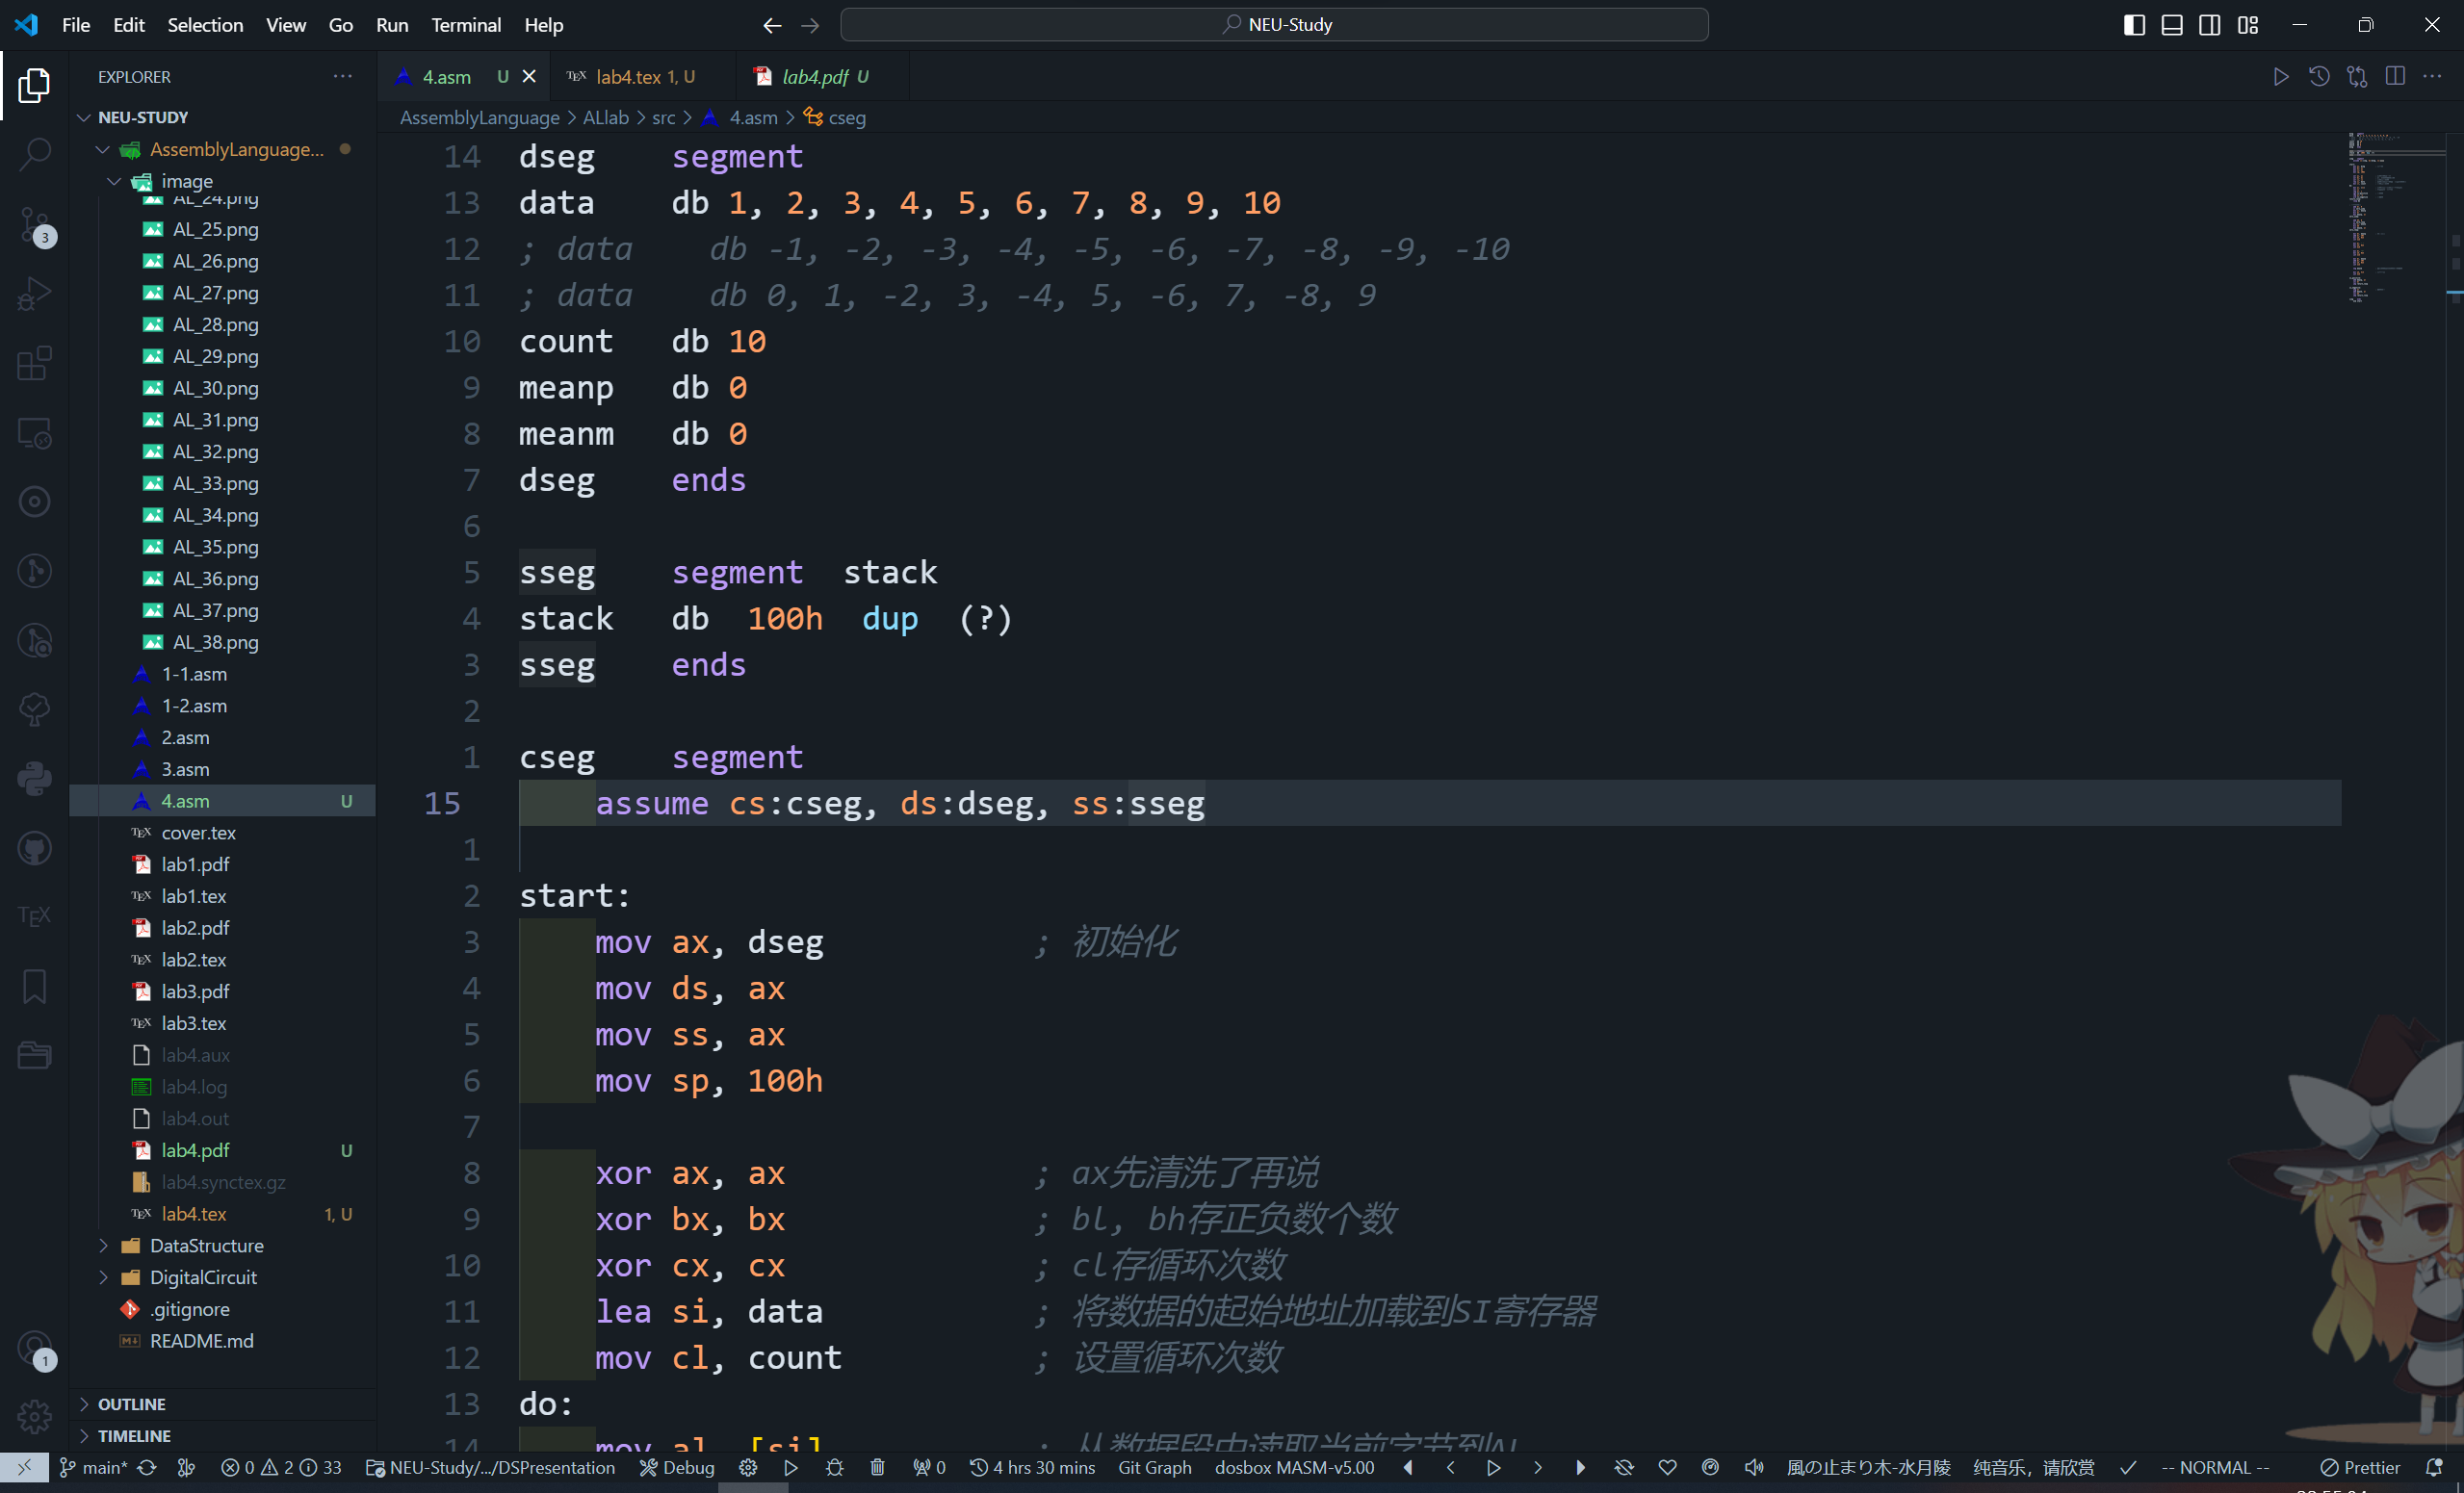
\includegraphics[width=1\textwidth]{image/AL_39.png}\end{center}
    \begin{center}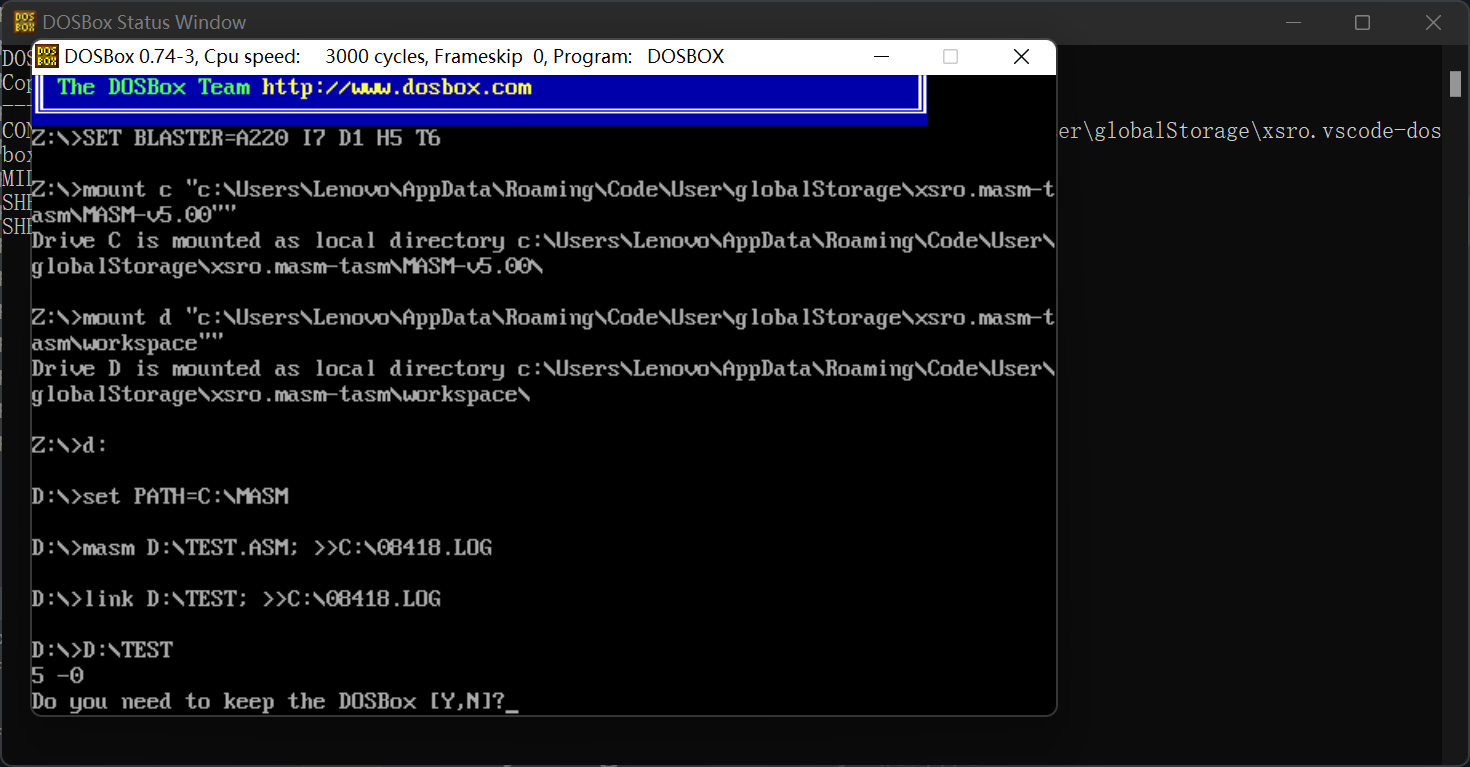
\includegraphics[width=1\textwidth]{image/AL_40.png}\end{center}
    全部负数：
    \begin{center}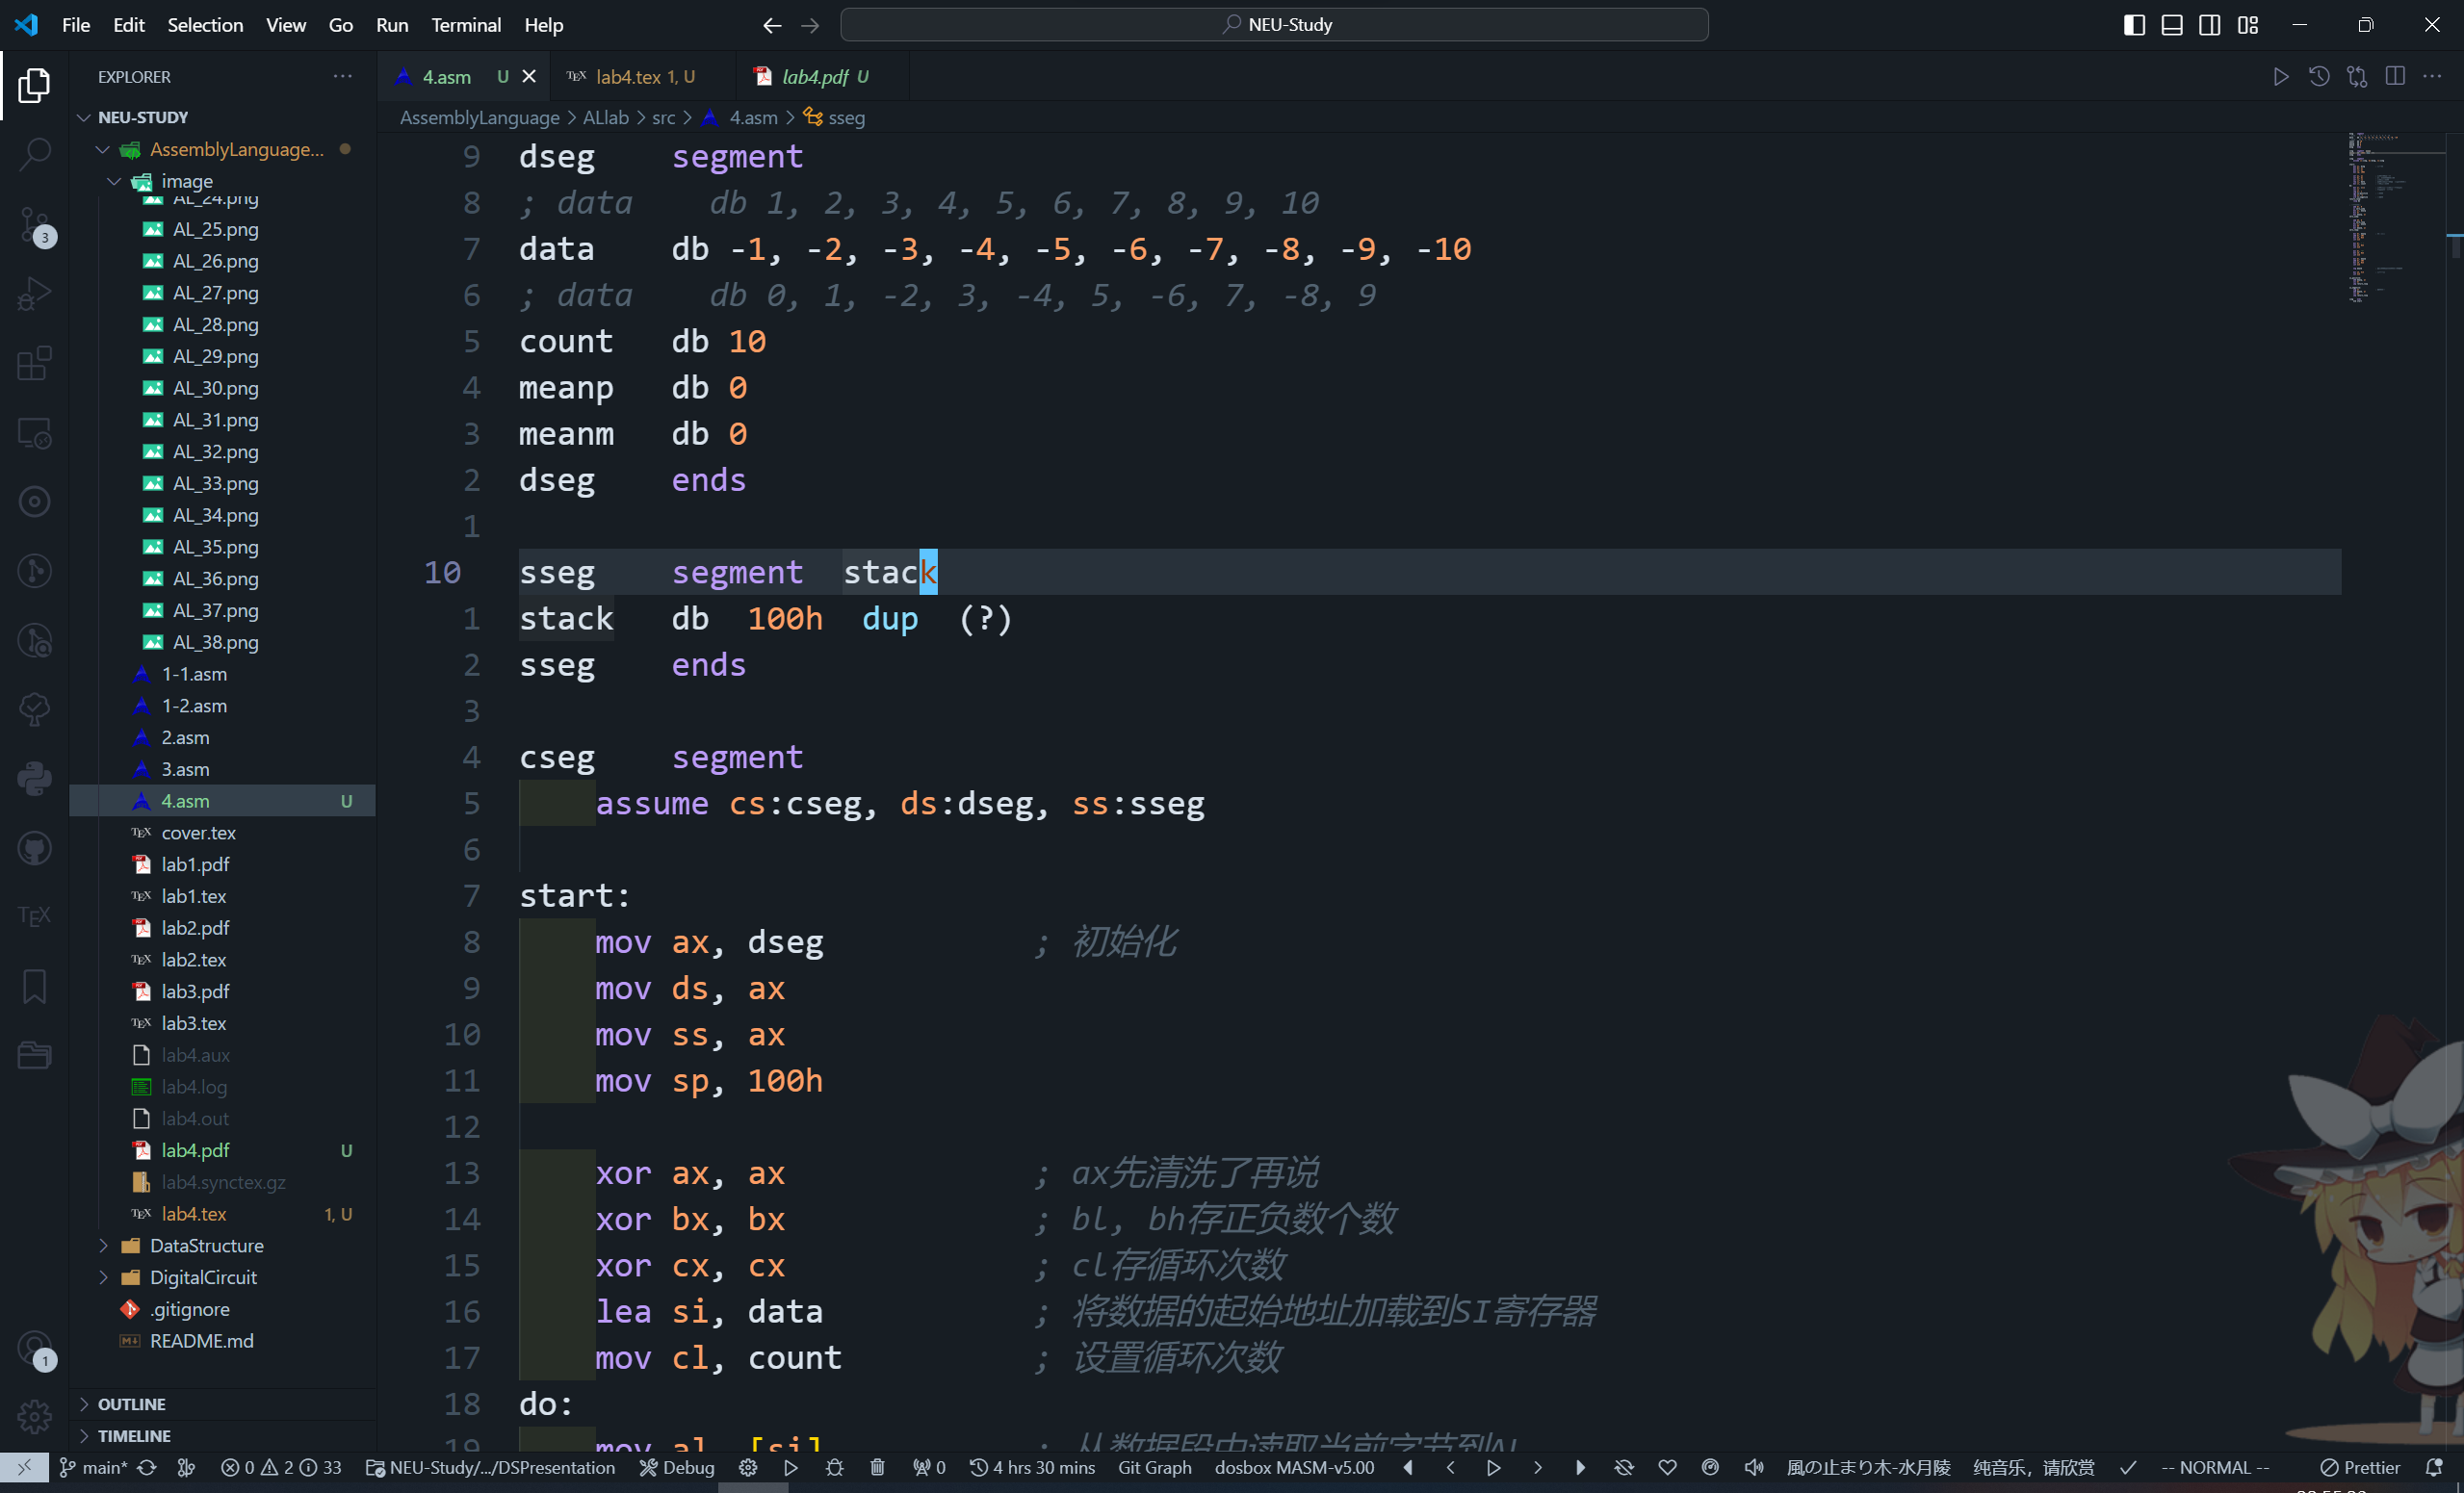
\includegraphics[width=1\textwidth]{image/AL_41.png}\end{center}
    \begin{center}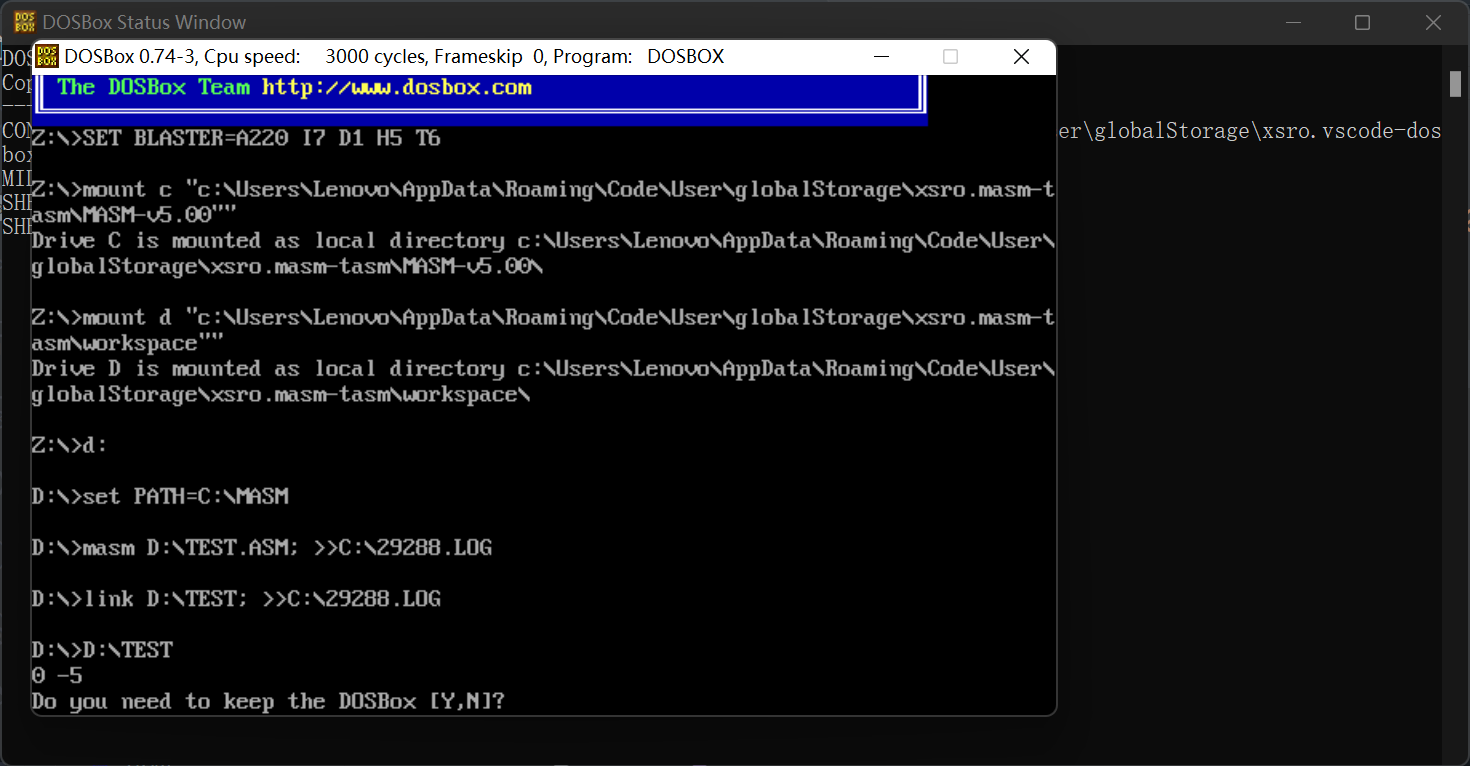
\includegraphics[width=1\textwidth]{image/AL_42.png}\end{center}
    有正数，负数和0：
    \begin{center}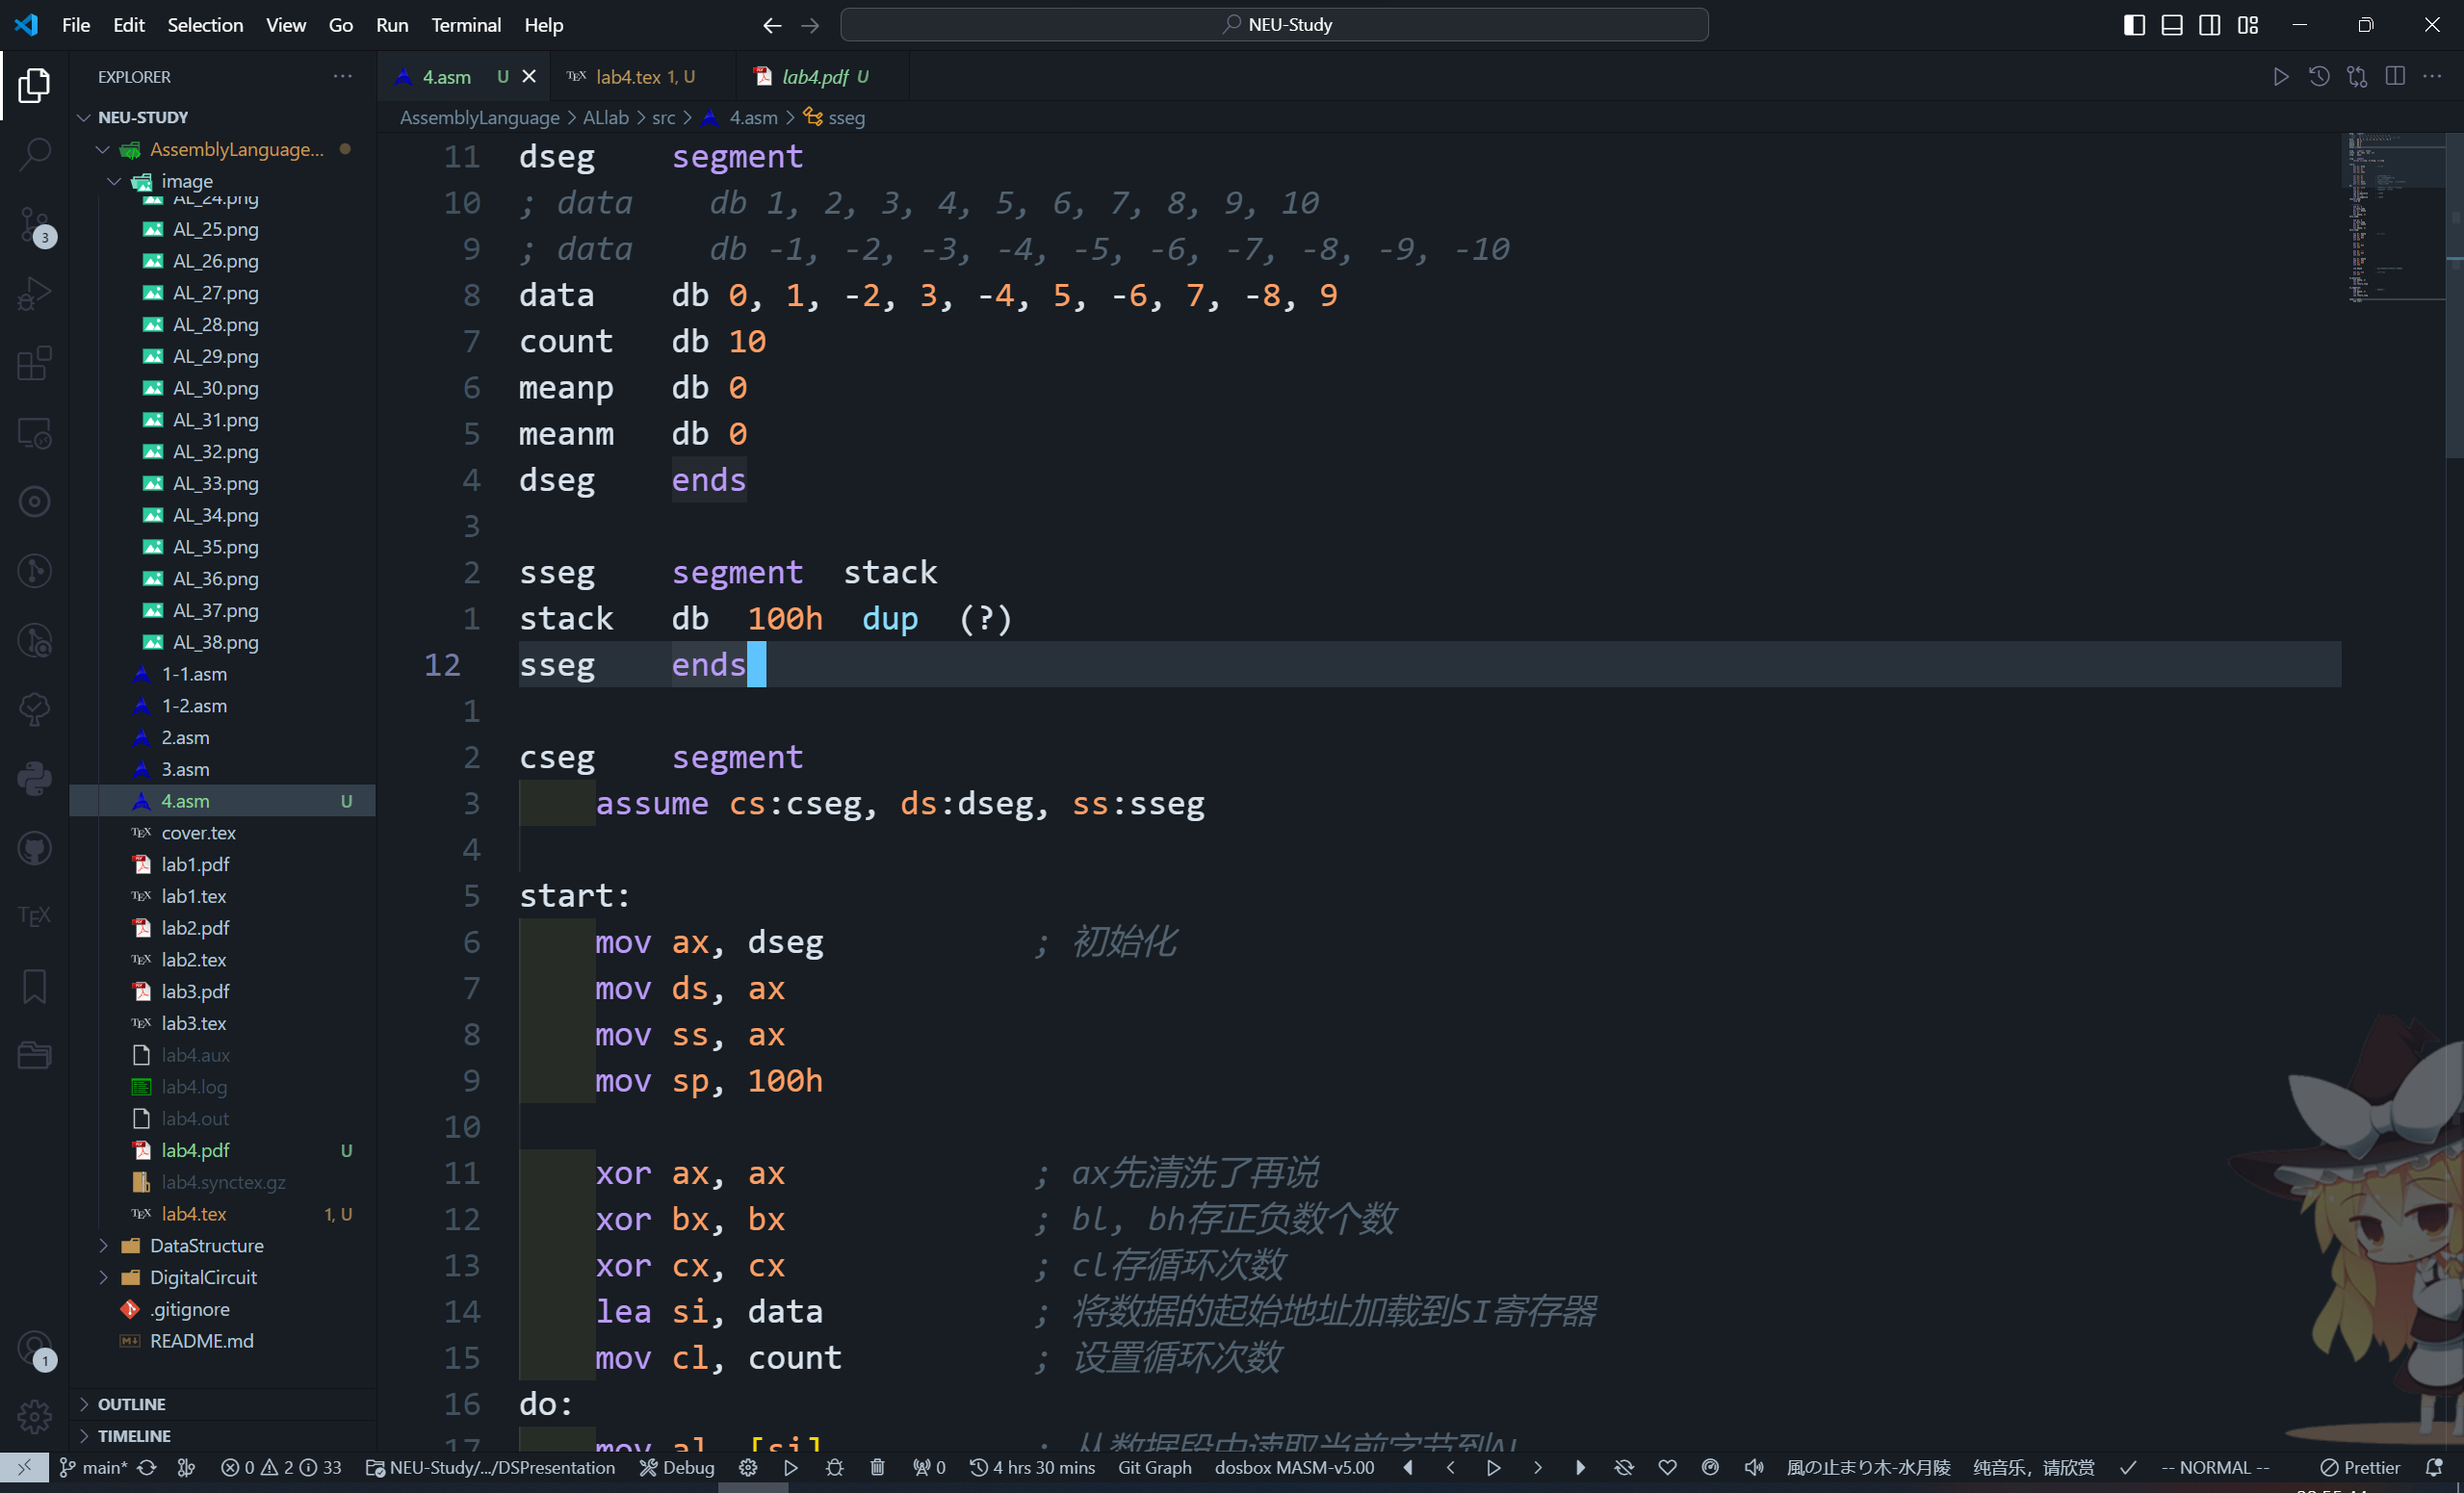
\includegraphics[width=1\textwidth]{image/AL_43.png}\end{center}
    \begin{center}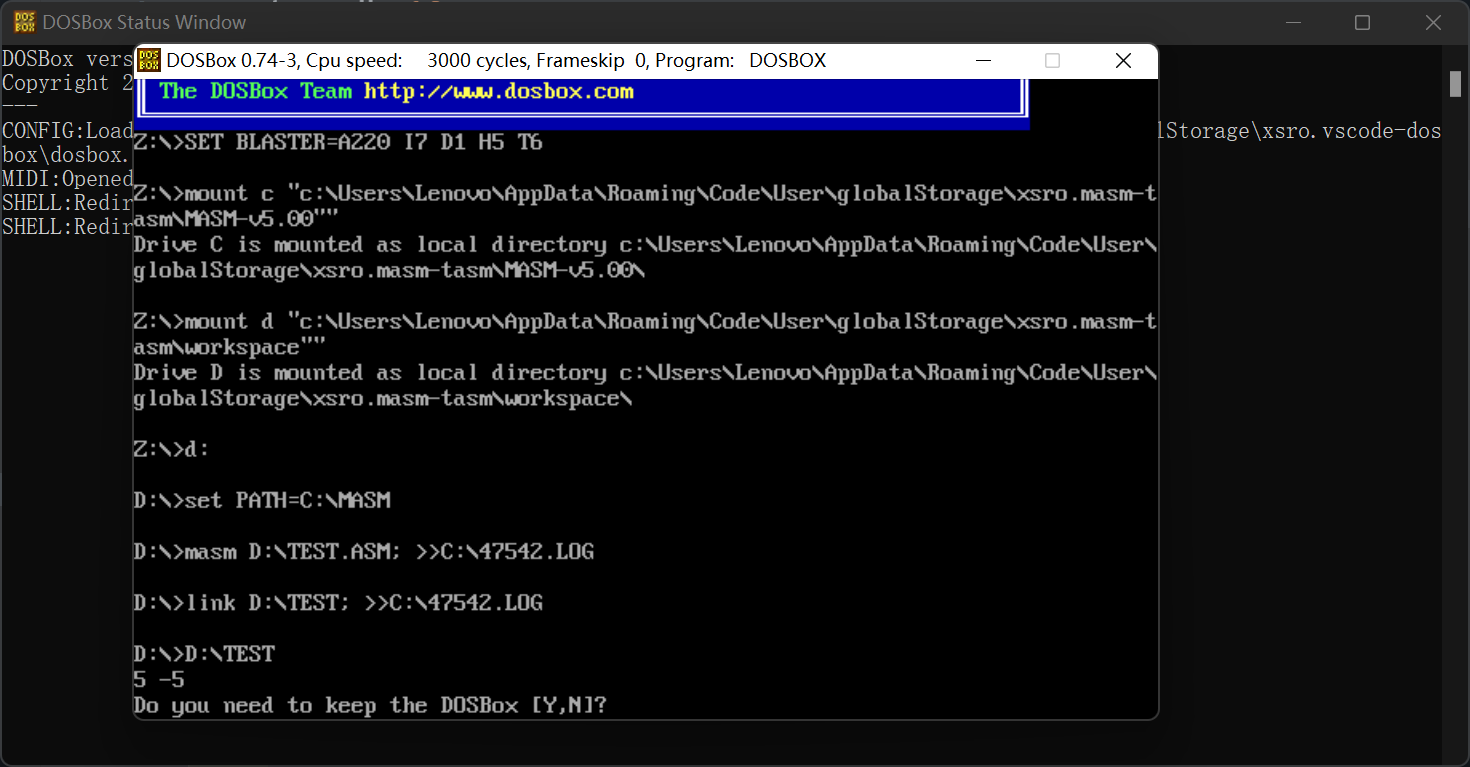
\includegraphics[width=1\textwidth]{image/AL_44.png}\end{center}
    \subsection{流程图}
    \begin{center}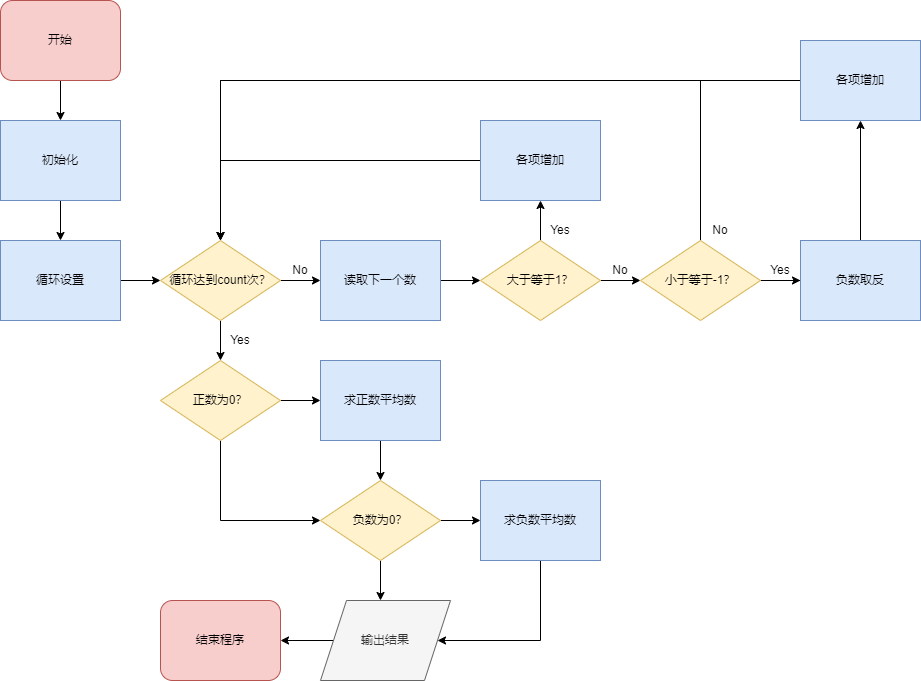
\includegraphics[width=1\textwidth]{image/AL_45.png}\end{center}

\section{心得体会}
通过这次汇编语言的实验，我深刻体会到了汇编语言在底层编程中的强大功能和精细操作的重要性。
在实验过程中，我不仅巩固了对数据段、堆栈和代码段等基本概念的理解，还实际操作了如何通过汇编语言直接与计算机硬件进行交互。

一开始，我在数据处理和循环控制结构的应用上遇到了一些困难。
特别是在实现循环来读取和处理数组数据时，如何有效地使用循环和条件分支来计算正负数的平均值成了一个挑战。
通过多次调试和修改程序，我逐渐理解了如何控制程序流和处理边界条件，比如如何避免除零错误。

此外，我也学习到了在程序中实现基本的输入输出操作的重要性。
使用DOS中断调用来输出计算结果是一个非常实践的过程，它让我了解到操作系统如何管理硬件资源并提供服务给应用程序。
这一部分的学习让我对操作系统的工作机制有了更直观的认识。

在解决问题的过程中，我发现详细的计划和预先的设计对于编程尤其重要。
在写代码之前，仔细地设计每一部分的功能和接口，可以显著减少后期调试的工作量。
这一经验对我的编程习惯有了很大的影响，使我在面对复杂问题时能更加从容不迫。

总的来说，这次实验不仅提升了我的汇编语言编程能力，也加深了我对计算机科学基础知识的理解。
它让我更加认识到理论与实践相结合的重要性，并激发了我探索更深层次计算机知识的兴趣。
\begin{flushright}\begin{tabular}{rl}
    姓名: & 李俊洁\\
    班级: & 计算机2204 \\
    学号: & 20225443 \\
    课程: & 汇编语言程序设计 \\
    日期: & April 10, 2024 \\
    制作: & \LaTeX \\
    & 感谢您的批阅！
\end{tabular}\end{flushright}
\end{document}